
%\documentclass[manuscript]{acmart}
%\documentclass[acmsmall]{acmart}
%\settopmatter{printacmref=false}


\documentclass[
  a4paper,
  12pt,
  DIV=12,        % höherer Wert = schmalere Ränder, weniger Whitespacmi
  parskip=half,  % Absätze mit halbem Abstand statt Einzug
  headings=small % kleinere Überschriften, weniger vertikaler Abstand
]{scrartcl}

%\documentclass[a4paper,11pt]{scrartcl}
%\documentclass[a4paper,11pt]{report}
%\documentclass[a4paper,12pt]{book}
\usepackage[utf8]{inputenc}
\usepackage[german]{babel}
\usepackage[T1]{fontenc}
\usepackage{lmodern}
\usepackage[inkscapelatex=false]{svg}
% Texte im SVG von Inkscape setzen lassen, nicht durch die Dokumentschrift ersetzen
\svgsetup{inkscapelatex=false}
\usepackage{amsmath}
\usepackage{caption}
\usepackage{gensymb}
\usepackage{microtype}
\usepackage{longtable}
\usepackage{tabularx}   % Spalten, die die restliche Zeilenbreite auffüllen (X-Spalte)
\usepackage{booktabs}   % \toprule \midrule \bottomrule (in mobrob_table.tex verwendet)
\usepackage{wrapfig}    % Textumfluss um Abbildungen

\usepackage[citecolor=black, colorlinks=true, linkcolor=black, urlcolor=blue]{hyperref}


%\usepackage{geometry}
\usepackage{siunitx}
%\geometry{margin=2.5cm}


\usepackage{amsthm}
\usepackage{mdframed}
\usepackage{enumitem}
\usepackage{eurosym}

\newmdtheoremenv{theorem}{Theorem}

\theoremstyle{definition}
\newmdtheoremenv{derivation}{Derivation}


%\mdfdefinestyle{leftline}{
%    topline=false, bottomline=false, rightline=false,
%    linewidth=2pt, linecolor=gray
%}
\theoremstyle{definition}
\newmdtheoremenv[style=leftline]{myalgorithm}{Algorithm}




%\usepackage{fancyvrb}







\let\Bbbk\relax
\usepackage{amssymb}


\usepackage{yfonts}

\usepackage{kvmap}

%\usepackage[
%    backend=biber,
%    style=alphabetic,
%    sortlocale=de_DE,
%    natbib=true,
%    %url=false,
%    doi=true,
%    %eprint=false
%]{biblatex}
%\addbibresource{Literaturrecherche-Stefan-Etringer/algo-references.bib}

%\usepackage[
%    backend=biber,
%    style=alphabetic,
%    sortlocale=de_DE,
%    natbib=true,
%    %url=false,
%    doi=true,
%    %eprint=false
%]{biblatex}
%\addbibresource{Literaturrecherche-Dennis/mobrob_references.bib}

\usepackage[autostyle=true,german=quotes]{csquotes}
\usepackage{trfsigns} %fourier transform arrow
\usepackage{mathrsfs} %fourier F
\usepackage{commath}

\usepackage{pgfplots}
\pgfplotsset{compat=1.18}

\usepackage{xcolor}
\usepackage{listings}
\usepackage[european]{circuitikz}
\ctikzset{tripoles/european not symbol=ieee circle}

%\usepackage[shading]{moeptikz}
%\moeptikzset{shading=true}

%\usepackage{german,longtable}

\usepackage{xcolor}
\usepackage{color}
\usepackage{url}

\usepackage{xfrac}

\usepackage{listings}
\usepackage{verbatimbox}

\usepackage{algorithm}
\usepackage{algpseudocode}

\usepackage{multirow}
\usepackage{float}
\usepackage{pdflscape}   % einzelne Querformatseiten (im PDF gedreht)

%%%% TIKZ

\usepackage{tikz}

\usepackage{pgfplots}
\usetikzlibrary{calc,
trees,positioning,arrows,
chains,shapes.geometric,
decorations.pathreplacing,
decorations.pathmorphing,shapes,
matrix,shapes.symbols,
plotmarks}
%\tikzexternalize[prefix=figures/]

%\tikzset{%
%  block/.style    = {draw, thick, rectangle, minimum height = 3em,
%    minimum width = 3em},
%  sum/.style      = {draw, circle, node distance = 2cm}, % Adder
%  input/.style    = {coordinate}, % Input
%  output/.style   = {coordinate} % Output
%}
% Defining string as labels of certain blocks.
%\newcommand{\suma}{\Large$+$}
%\newcommand{\multa}{\Large$\times$}
%\newcommand{\inte}{$\displaystyle \int$}
%\newcommand{\derv}{\huge$\frac{d}{dt}$}

\usetikzlibrary{arrows,automata,positioning}
%\usepackage{automata}


%%% END TIKZ

\usepackage[section]{placeins}

\usepackage{textcomp}


\usepackage{listings}
\usepackage{verbatimbox}

\usepackage{bold-extra}

\usepackage{framed}

%\usepackage{fancyhdr}
%\pagestyle{fancy}
%\lhead{\leftmark}
%\chead{}
%\rhead{}
%\lfoot{}
%\cfoot{\thepage}
%\rfoot{}
%\renewcommand{\headrulewidth}{0.2pt}
%\renewcommand{\footrulewidth}{0.2pt}



\newcommand{\Z}{\mathbb{Z}}
\newcommand{\R}{\mathbb{R}}
\newcommand{\C}{\mathbb{C}}
\newcommand{\N}{\mathbb{N}}
\newcommand{\SqrtNy}{$\sqrt{\textsc{Ny}}$}
\newcommand{\conj}{\overline}
\newcommand{\Kset}{\textswab{K}}
\newcommand{\Qset}{\textswab{Q}}
\newcommand{\ceil}[1]{\left\lceil #1 \right\rceil}
\newcommand{\floor}[1]{\left\lfloor #1 \right\rfloor}
\newcommand{\sorted}[1]{\textsc{sort}\left\lbrace #1 \right\rbrace}
\newcommand{\SNRgain}{a_{SNR}}
\newcommand{\EQgain}{a_{EQ}}
\newcommand{\SIRgain}{a_{SIR}}
\newcommand{\SNIRgain}{a_{SINR}}
\newcommand{\SNR}{\textsc{SNR}}
\newcommand{\CIRgain}{a_{CIR}}
\newcommand{\CINRgain}{a_{CINR}}
\newcommand{\CNR}{\textsc{CNR}}
\newcommand{\CINR}{\textsc{CINR}}
\newcommand{\HPAModel}{ Hughes 1177H TWTA }
\newcommand{\bigO}{\mathcal{O}}
\newcommand{\CopWinCompl}{2.375377}
\newcommand{\IBO}{\textsc{IBO}}
\newcommand{\OBO}{\textsc{OBO}}
\newcommand{\spacepage}{\newpage\null\thispagestyle{empty}\newpage}
\newcommand{\satcom}{ SatCom }
\newcommand{\db}{~\text{dB}}


\definecolor{mGreen}{rgb}{0,0.6,0}
\definecolor{mGray}{rgb}{0.5,0.5,0.5}
\definecolor{mPurple}{rgb}{0.58,0,0.82}
\definecolor{backgroundColour}{rgb}{0.95,0.95,0.92}

\lstdefinestyle{CStyle}{
    backgroundcolor=\color{backgroundColour},
    commentstyle=\color{mGreen},
    keywordstyle=\color{magenta},
    numberstyle=\tiny\color{mGray},
    stringstyle=\color{mPurple},
    basicstyle=\footnotesize,
    breakatwhitespace=false,
    breaklines=true,
    captionpos=b,
    keepspaces=true,
    numbers=left,
    numbersep=5pt,
    showspaces=false,
    showstringspaces=false,
    showtabs=false,
    tabsize=2,
    language=C
}

\lstdefinelanguage{VHDL}{
  morekeywords=[1]{library,use,all,entity,is,port,in,out,end,architecture,of,begin,process,if,then,else,elsif,when,others,signal,variable,wait,for,loop},
  morecomment=[l]--,
  morestring=[b]",
  sensitive=true
}

\lstset{
  language=VHDL,
  basicstyle=\ttfamily\small,
  keywordstyle=\color{blue},
  commentstyle=\color{gray},
  stringstyle=\color{red},
  numbers=left,
  numberstyle=\tiny,
  stepnumber=1,
  numbersep=8pt,
  frame=single,
  breaklines=true,
  captionpos=b
}

\lstset{numbers=none}

%\newcounter{example}
%\renewcommand{\theexample}{\thesection.\arabic{example}}


% Default fixed font does not support bold face
\DeclareFixedFont{\ttb}{T1}{txtt}{bx}{n}{12} % for bold
\DeclareFixedFont{\ttm}{T1}{txtt}{m}{n}{12}  % for normal

% Custom colors
\usepackage{color}
\definecolor{deepblue}{rgb}{0,0,0.5}
\definecolor{deepred}{rgb}{0.6,0,0}
\definecolor{deepgreen}{rgb}{0,0.5,0}

\usepackage{listings}

% Python style for highlighting
\newcommand\pythonstyle{\lstset{
language=Python,
basicstyle=\ttm,
morekeywords={self},              % Add keywords here
keywordstyle=\ttb\color{deepblue},
emph={MyClass,__init__},          % Custom highlighting
emphstyle=\ttb\color{deepred},    % Custom highlighting style
stringstyle=\color{deepgreen},
frame=tb,                         % Any extra options here
showstringspaces=false
}}


% Python environment
\lstnewenvironment{python}[1][]
{
\pythonstyle
\lstset{#1}
}
{}

% Python for external files
\newcommand\pythonexternal[2][]{{
\pythonstyle
\lstinputlisting[#1]{#2}}}

% Python for inline
\newcommand\pythoninline[1]{{\pythonstyle\lstinline!#1!}}





\nocite{*}


\begin{document}
%\pagenumbering{roman}



\title{Coasterbot}
\subtitle{Phasenpaper M0}
\author{Gereon Such}
%\email{gereonsuch@suchdsp.com}
%\affiliation{
%  \institution{Wilhelm Büchner University of Applied Sciences}
%  \department{Computer Engineering}
%  \city{Hof}
%  \country{Germany}
%}



\begin{titlepage}
  \begin{center}
    {\large Wilhelm Büchner University of Applied Sciences} \\[0.3em]

    {\normalsize Projektseminar Master}
\vspace{5em}

    {\LARGE\bfseries Coasterbot} \\[0.5em]

    {\large Ressourcen- und Kostenplan} \\[1em]

    {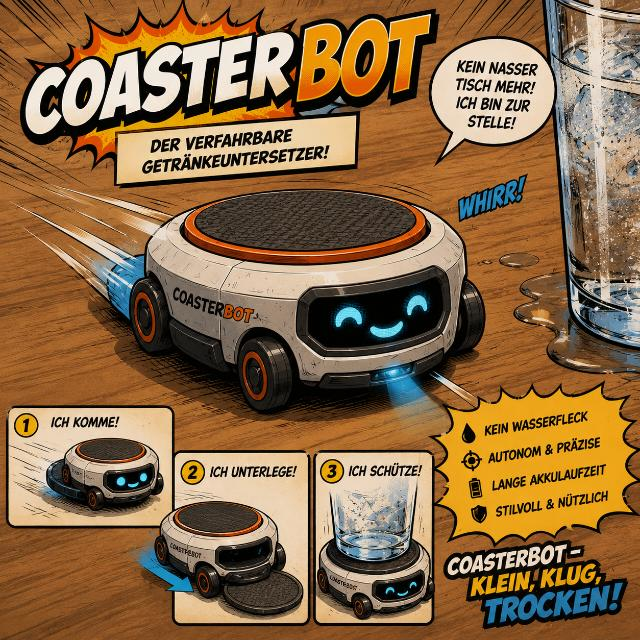
\includegraphics[width=0.38\textwidth]{coasterbot.png}} \\[1em]

\vspace{4em}

    {\normalsize
\begin{tabular}{ll}
Dennis Borutta, B. Eng & dennis.borutta@outlook.com\\
Stefan Etringer, B. Eng & mail@stefan.works\\
Gereon Such, M. Sc. & gereonsuch@gmail.com\\
\end{tabular}
    }
  \end{center}


\end{titlepage}


% einleitung preambel etc.


% Versionshistorie des Dokuments -- eigene Seite direkt nach dem Titelblatt
\section*{Versionshistorie}

\begin{tabularx}{\textwidth}{@{}clp{2.6cm}X@{}}
\toprule
\textbf{Version} & \textbf{Datum} & \textbf{Bearbeiter} & \textbf{Änderungen}\\
\midrule
1 & 30.07.2026 & Such & Erstfassung des Resourcen- und Kostenplan auf Basis Netzplan\\
2 & 30.07.2026 & Such & Aufwandschätzung tabelarisch direkt in Kosten gerechnet, nicht nur Stunden.\\
3 & 31.07.2026 & Such & Werkzeuge über Gemeinkosten berücksichtigt. \\
\bottomrule
\end{tabularx}


\newpage

\tableofcontents

\newpage

\section{Allgemeines}

Der Coasterbot ist ein Studienprojekt und als solches sind Arbeitsstunden und Aufwand für gewöhnlich nicht mit Arbeitsstunden gegenzurechnen, da auch eine akademische Lernkurve zu berücksichtigen ist. Dennoch soll dieses Dokument im Sinne eines Startups auch die Arbeitszeit als primäre Kosten des Projekts erfassen. 

Die aufgeführten Arbeitsstunden sind am Projektstrukturplan und der Vorgangsliste aus Meilenstein M0 ausgerichtet. Laut diesen war eine Kostenkalkulation eigentlich mit Arbeitspaket 3040 eingeplant, sollte aber für M0 vorgezogen werden. 

\textbf{Hinweis}: Der Plan folgt der klassischen ingenieurmäßigen Projektkalkulation mit WBS-basierter Aufwandsschätzung und Stundensatzermittlung nach dem Zuschlagsverfahren. 


\subsection{Rahmen und Annahmen}


\begin{tabularx}{\textwidth}{lX@{}}
\toprule
\textbf{Punkt} & \textbf{Annahme} \\
\midrule
Team & 3 Ingenieure \\
Charakter & Studien-/Nebenprojekt, kalkuliert wie ein Unternehmen \\
Projektlaufzeit & 15.07.2026 – 16.10.2026 ($\approx$ 13,5 Wochen) \\
Ziel & Prototyp \textbf{Maturity Level 1} \\
Werkzeuge & vorhanden (keine Anschaffung; im Gemeinkostensatz berücksichtigt) \\
Software & vollständig Open Source $\rightarrow$ 0 € Lizenzkosten \\
Material & muss beschafft werden; bisher ca. 40 \euro{ } ausgegeben \\
3D-Druck & Plattform/Chassis steht noch aus \\
\bottomrule
\end{tabularx}


Zwei Sichten werden getrennt ausgewiesen:

\begin{itemize}
\item \textbf{Unternehmenssicht (Vollkosten)}: Personal wird mit kalkulatorischem Stundensatz bewertet (was das Projekt „kosten würde").
\item \textbf{Reale Auslage}: nur tatsächliche Ausgaben der Gruppe (Material) wird berücksichtigt. Als Ingenieursstudenten mit praktischen Fähigkeiten sind Werkzeuge für einen Prototypen hinreichend vorhanden, Softwareseitig wird Open Source verwendet. 
\end{itemize}




\section{Ressourcenplan}

\subsection{Personal}

\begin{tabularx}{\textwidth}{llX@{}}
\toprule
\textbf{Rolle} & \textbf{Anzahl} & \textbf{Einsatz} \\
\midrule
Ingenieur & 3 & nebenberuflich über gesamte Projektlaufzeit \\
\bottomrule
\end{tabularx}



\subsection{Sachmittel}


\begin{tabularx}{\textwidth}{X@{}lr}
\toprule
\textbf{Ressource} & \textbf{Status} & \textbf{Kosten} \\
\midrule
Werkzeuge (Werkstatt, Lötausrüstung, 3D-Drucker) & vorhanden & 0 \euro \\
Software (IDE, Simulation, FreeCAD, KiCAD) & Open Source & 0 \euro \\
Elektronik/Mechanik-Material Prototyp & zu beschaffen & siehe Kap.  \ref{matkostenprototyp} \\
3D-Druck-Filament & zu beschaffen & siehe Kap.  \ref{matkostenprototyp} \\
Rechner/Arbeitsplatz/IT & vorhanden & 0 \euro \\
\bottomrule
\end{tabularx}


\section{Stundensatzermittlung per Zuschlagskalkulation}



Kalkulatorischer Stundensatz eines Ingenieurs, hergeleitet über Personal(voll)kosten, produktive Stunden, Gemeinkosten sowie Wagnis und Gewinn.



\subsection{Produktive Stunden pro Jahr}


\begin{tabularx}{\textwidth}{X@{}r}
\toprule
\textbf{Position} & \textbf{Stunden} \\
\midrule
Bruttoarbeitszeit (52 Wo × 40 h) & 2.080 \\
- Urlaub (30 AT) & -240 \\
- Feiertage ($\approx$ 11 Tage) & -88 \\
 - Krankheit ($\approx$ 8 AT) & -64 \\
 = Anwesenheit & 1.688  \\
 x Produktivitätsgrad $\approx$ 83 \% (verrechenbar) & \textbf{$\approx$ 1.400} \\
\bottomrule
\end{tabularx}


\subsection{Stundensatz}


\begin{tabularx}{\textwidth}{X@{}r}
\toprule
\textbf{Position} & \textbf{Stunden} \\
\midrule
Jahresbruttogehalt Ingenieur (Annahme) & 54.000 \euro \\
+ Arbeitgeber-Lohnnebenkosten (21 \%) & 11.340 € \\
\textbf{= Arbeitgeber-Personalkosten p. a.} & \textbf{65.340 \euro} \\
÷ produktive Stunden p. a. & 1.400 h \\
\textbf{= Personalkostensatz}  & \textbf{46,70 \euro /h} \\
+ Gemeinkostenzuschlag (90 \% – Arbeitsplatz, IT, Werkzeuge/Abschreibung, Verwaltung, Leitung) & 42,00 \euro /h \\
\textbf{= Selbstkostensatz (Vollkosten)} & \textbf{$\approx$ 89 \euro /h} \\
+ Wagnis und Gewinn (12 \%) & 10,60 €/h \\
\textbf{= Angebots-/Verrechnungssatz}  & \textbf{$\approx$ 100 \euro /h} \\
\bottomrule
\end{tabularx}

\begin{itemize}
\item Für die interne Projektbewertung wird der \textbf{Selbstkostensatz 89 \euro /h} verwendet. 
\item Der Verrechnungssatz 100 €/h zeigt den Marktwert (Opportunitätskosten).
\item Alle Gehalts-/Zuschlagswerte sind Annahmen und in der Tabelle leicht anpassbar.
\item Privat beschaffte Werkzeuge werden über die Gemeinkosten berücksichtigt. Da die Projektdauer begrenzt ist sind diese Kosten ohnehin nicht erheblich: Bei privatem Werkzeug im Wert von 2000 \euro, einer Nutzungsdauer von 6 Jahren und einem Nutzungsgrad von 25 \% ergibt sich eine kalkulatorische Abschreibung über die Projektzeit von 3.5 Monaten von $ 2000 \cdot \sfrac{3.5}{6\cdot 12\cdot4} = 24 $ \euro. 
\end{itemize}



\section{Aufwandsschätzung je Arbeitspaket}

Personenstunden je Arbeitspaket entsprechend Netzplan. Die dortige Dauer ist Vorgangsdauer in Tagen, somit wird der \textbf{Personalaufwand} geschätzt.

\begin{tabularx}{\textwidth}{lX@{}rr}
\toprule
\textbf{AP} & \textbf{Beschreibung} & \textbf{Aufwand [h]} & \textbf{Kosten} \\
\midrule
1001 & Steckbriefdefinition & 4 & 356 \euro \\
1002 & Projektorganisation und Planung & 12 & 1068 \euro \\
1010 & Algorithmik recherchieren & 20 &1780 \euro \\
1020 & Marktsichtung durchführen & 20 &1780 \euro \\
1030 & Stand Mobile Robotik recherchieren & 20 &1780 \euro \\
101 & Dokumente zusammentragen & 6 & 534 \euro\\
2010 & Anwendungsfälle definieren & 10 & 890 \euro\\
2020 & Maturity Level definieren & 10 & 890 \euro\\
2030 & Lastenheft erstellen & 24 & 2136 \euro\\
3010 & Testfälle definieren & 16 & 1424 \euro\\
3020 & Sensorik/Aktorik auswählen & 20 & 1780 \euro\\
3030 & Softwarearchitektur erarbeiten & 24 & 2136 \euro\\
3040 & Kostenkalkulation durchführen & 12 & 1068 \euro\\
3050 & Pflichtenheft erstellen & 30 & 2670 \euro\\
201 & Dokumente zusammentragen & 4 & 356 \euro\\
4010 & Bauteile beschaffen & 10 & 890 \euro\\
4020 & Softwaretest erstellen & 40 & 3560 \euro\\
4030 & Software implementieren & 120 & 10680 \euro\\
4040 & Prototyp aufbauen & 50 & 4450 \euro\\
5000 & Test durchführen & 40 & 3560 \euro\\
6000 & Maturity Level feststellen & 12 & 1068 \euro\\
301 & Dokumente zusammentragen & 6 & 534 \euro\\
401 & Endbericht erstellen und abgeben & 40 & 3560 \euro\\
7000 & Präsentation ausarbeiten & 30 & 2670 \euro\\
& \textbf{Summe} & 580 & 51620 \euro\\
\bottomrule
\end{tabularx}

\hspace{4cm}

\subsection{Aufwand je Phase}

\begin{tabularx}{\textwidth}{X@{}rrr}
\toprule
\textbf{Phase} & \textbf{Aufwand [h]} & \textbf{Kosten} & \textbf{Anteil} \\
\midrule
Initialisierung und Recherche (10xx, 101) & 82 & 7298 \euro& 14 \% \\
Anforderungen / Lastenheft (20xx) & 44 & 3916 \euro & 8 \% \\
Konzept und Pflichtenheft (30xx, 201) & 106 & 9434 \euro & 18 \% \\
Realisierung (40xx) & 220 & 19580 \euro & 38 \% \\
Test und Abschluss (5000–7000, 301, 401) & 128 & 11392 \euro & 22 \% \\
\textbf{Gesamt} & \textbf{580} & \textbf{51620 \euro } &  100 \% \\
\bottomrule
\end{tabularx}

\begin{itemize}
\item Kapazitätsabgleich: 580 h ÷ 3 Personen $\approx$ \textbf{193 h/Person} über 13,5 Wochen 
$\approx$ \textbf{14–15 h/Woche/Person}. 
\end{itemize}



\section{Materialkosten der Prototyp-Phase}
\label{matkostenprototyp}

\begin{itemize}
\item 3D-Druck als Eigenfertigung angesetzt
\item 3d-Drucker sowie weitere Werkzeuge gelten als vorhanden im Team. 
\end{itemize}


\begin{tabularx}{\textwidth}{X@{}r}
\toprule
\textbf{Position} & \textbf{Betrag} \\
\midrule
Bereits beschafft (Sensoren, TT-Motoren, TB6612-Treiber, Servos lt. Empfehlung) & 40 \euro \\
3D-Druck Chassis/Plattform (Filament inkl. Iteration/Ausschuss) & 15  \euro \\
Ergänzung ML-1-Vollständigkeit (Encoder/IMU, zusätzl. Ultraschall, Microswitches, Status-LED/Buzzer, Not-Aus) & 90  \euro \\
Energieversorgung (Akkupack/Batteriehalter, Hauptschalter) & 15  \euro \\
Verbrauchsmaterial/Kleinteile (Kabel, Stecker, Lötzinn, Schrauben, Standoffs, Kabelbinder, Breadboard/Lochraster) & 20  \euro \\
\textbf{Zwischensumme} & \textbf{180 \euro} \\
Risikopuffer 15 \% & 27 \euro \\
\textbf{Materialosten gesamt} & $\approx$ 207 \euro \\
\bottomrule
\end{tabularx}



\section{Kostenzusammenfassung (Vollkosten)}

\begin{tabularx}{\textwidth}{X@{}lr}
\toprule
\textbf{Kostenart} & \textbf{Berechnung} & \textbf{Betrag} \\ 
\midrule
\textbf{Personalkosten} & 580 h × 89 €/h & \textbf{51.620} \euro \\
\textbf{Materialkosten} & siehe Kap. \ref{matkostenprototyp} & \textbf{207 \euro} \\
Software (Open Source) & - & \textbf{0 €} \\
Werkzeuge (vorhanden) & - & \textbf{0 €} \\
\textbf{Projektkosten gesamt (Vollkosten)} & & \textbf{$\approx$ 51.827 \euro} \\
\bottomrule
\end{tabularx}


%\newpage
%\section{Anhänge}

%\appendix

%acm bullshit
%\bibliographystyle{ACM-Reference-Format}
%\bibliography{quellen}

% normal scr article
%\printbibliography[title={Literaturverzeichnis}]

%\listoffigures


%\newpage
%\chapter*{References}
%\addcontentsline{toc}{chapter}{References}
%\printbibliography[heading=none]

\end{document}
